199. \begin{figure}[ht!]
\center{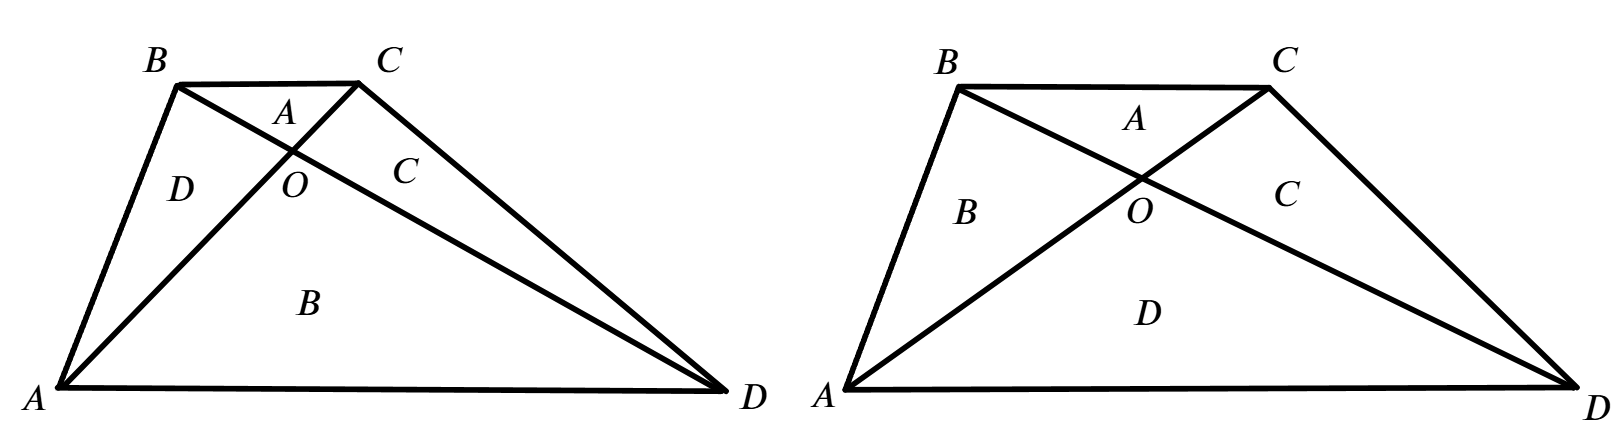
\includegraphics[scale=0.35]{g9-199.png}}
\end{figure}\\
Возможны два разных случая расположения площадей: площади $A$ и $B$ могут быть в трапеции соседними или противоположными.

Первый случай: они противоположны. Треугольники $AOD$ и $BOC$ подобны по двум углам, отношение их площадей равно $8:4=2,$ значит коэффициент подобия равен $\sqrt{2}$ и $AO:CO=\sqrt{2}:1.$ У треугольников $ABO$ и $BCO$ общая высота из точки $B,$ значит их площади относятся как основания, к которым эта высота проведена, и $\cfrac{S_{\Delta ABO}}{S_{\Delta BOC}}=\cfrac{AO}{CO}=\sqrt{2},$ откуда $S_{\Delta ABO}=\sqrt{2}\cdot4=4\sqrt{2},$ аналогично и $S_{\Delta CBO}=4\sqrt{2}.$ Поэтому в данном случае площадь трапеции $ABCD$ равна $4+8+4\sqrt{2}+4\sqrt{2}=12+12\sqrt{2}.$

Второй случай: они соседние. Тогда аналогично первому случаю имеем соотношение $\cfrac{AO}{OC}=\cfrac{S_{\Delta ABO}}{S_{\Delta BOC}}=8:4=2,$ а значит треугольники $AOD$ и $BOC$ подобны с коэффициентом 2 и $S_{\Delta AOD}=4S_{\Delta BOC}=4\cdot4=16.$ Так как $OD:BO=2,$ то и $S_{\Delta COD}=4\cdot2=8,$ а значит площадь всей трапеции $ABCD$ равна $4+8+8+16=36.$\\
